\section{Observations}
\label{sec:observations}

Roughly 16K total exposures were acquired during the ComCam on-sky campaign from 24 October 2024 to 11 December 2024.
\tabRef{img_type} summarizes the distribution of visits, disaggregated by \texttt{img\_type}.
The visits include more than 10K exposures for active optics system (AOS) commissiong (roughly one-third each of intra-focal, extra-focal, and in-focus images), more than 2K bias and dark calibration frames, and more than 2K visits for Science Pipelines commissioning.

\begin{table*}
    \centering
    \begin{tabular}{@{}lll@{}}
    \textbf{\texttt{img\_type}} & \textbf{Number of Visits} & \textbf{Notes} \\
    \hline
    ACQ & 5261 & Includes in-focus visits for AOS commissioning \\
    BIAS & 1432 & Bias frames for calibration \\
    CWFS & 5169 & Curvature wavefront sensing for AOS commissioning \\
    DARK & 1153 & Dark frames for calibration \\
    ENGTEST & 169 & Includes CBP commissioning \\
    FLAT & 37 & \\
    FOCUS & 534 & Focus sequences \\
    OBJECT & 2144 & Mostly visits for Science Pipelines commissioning \\
    STUTTERED & 61 & Stuttered imaging \\
    \end{tabular}
    \caption{Distribution of visits by image type (\texttt{img\_type}) during the ComCam on-sky campaign.}
    \label{tab:img_type}
\end{table*}

\subsection{Observations for Science Pipelines Commissioning}

To maximize the utility of observations for Science Pipelines commissioning, the team acquired repeated observations distributed across multiple bands for a small set of fields across many nights to

\begin{itemize}
    \item test the internal astrometric and photometric calibration across a range of observing conditions and assemble large statistics,
    \item provide routine opportunities for testing difference image analysis and Prompt Processing framework, and
    \item accumulate upwards of 200 visits per band to evaluate deep coadds at roughly LSST WFD 10-year equivalent integrated exposure.
\end{itemize}

\tabRef{target_fields_pointing_centers} reports central pointing coordinates for seven target fields used for Science Pipelines commissioning during the ComCam on-sky campaign.
The fields were selected to collectively span a range of stellar densities, overlap external reference datasets to enable a broad range of science verification and validation studies, and span the breadth of the four primary LSST science themes.

The ComCam filter exchanger holds three filters at a time.
A typical observing epoch on a given target field consisted of 5-20 visits in each of the three loaded filters.
Nearly all of the visits for Science Pipelines commissioning used a single 30-second exposure, rather than 2 $\times$ 15-second ``snap'' exposures.

\figRef{comcam_ddf_coverage} and \figRef{comcam_ecliptic_coverage} show the coverage of the seven target fields.
Six of the fields used a pattern of random translational and rotational dithers within an 0.2 deg radius circle around the pointing center.
The rotational dithers were typically applied at the time of filter changes for operational efficiency, with small rotatoral dithers ($\sim1$ deg) applied between individual visits.

For the low ecliptic latitude field, the team used an alternative dither pattern to maximize the coverage of Solar System Objects and to facilitate testing Solar System Object linking across multiple nights.
The observations synthesized a 2 $\times$ 2 grid of ComCam pointings to cover a region roughly 1.3 deg $\times$ 1.3 deg (\figRef{comcam_ecliptic_coverage}).
The visits cycled between the four pointing centers in the grid, using small psuedo-random translational dithers to fill in chip gaps, with the goal of acquiring 3-4 visits at each pointing center in each band during in each observing epoch.

\tabRef{target_fields_band_coverage} provides a summary of the band coverage across the seven fields.
\figRef{comcam_ddf_psf_maglim} shows the resulting integrated depth, expressed in terms of the flux of an unresolved source that would be measured with signal-to-noise ratio $S/N = 5$, using the $r$ band as an example.

\figRef{comcam_science_day_obs} shows the distribution of science program observations across the ComCam on-sky campaign.
\figRef{comcam_science_day_obs_ecdfs} shows observations for the ECDFS field, which had the most consistent temporal sampling of the seven target fields during the campaign.

% 2394 = EDFS_comcam
% 5526 = Rubin_SV_095_-25
% 453 = 47Tuc
% 5063 = ECDFS
% 7611 = seagull
% 4016 = Fornax dSph
% 10463 = Rubin_SV_38_7

% 47 Tuc Globular Cluster (47 Tuc)
% (ra, dec) = (6.02, -72.08)

% Low Ecliptic Latitude Field (Rubin SV 38 7)
% (ra, dec) = (37.86, 6.98)

% Fornax Dwarf Spheroidal Galaxy (Fornax dSph)
% (ra, dec) = (40.00, -34.45)

% Extended Chandra Deep Field South (ECDFS)
% (ra, dec) = (53.13, -28.10)

% Euclid Deep Field South (EDFS)
% (ra, dec) = (59.10, -48.73)

% Low Galactic Latitude Field (Rubin SV 95 -25)
% (ra, dec) = (95.00, -25.00)

% Seagull Nebula (Seagull)
% (ra, dec) = (106.23, -10.51)

\begin{table*}
    \centering
    \begin{tabular}{@{}lcc@{}}
    \textbf{Target} & \textbf{RA} & \textbf{Declination} \\
     & \textit{deg} & \textit{deg} \\
    \hline
    47 Tuc Globular Cluster (47 Tuc)              & 6.02    & -72.08    \\
    Low Ecliptic Latitude Field (Rubin SV 38 7)   & 37.86   & 6.98      \\
    Fornax Dwarf Spheroidal Galaxy (Fornax dSph)  & 40.00   & -34.45    \\
    Extended Chandra Deep Field South (ECDFS)     & 53.13   & -28.10    \\
    Euclid Deep Field South (EDFS)                & 59.10   & -48.73    \\
    Low Galactic Latitude Field (Rubin SV 95 -25) & 95.00   & -25.00    \\
    Seagull Nebula (Seagull)                      & 106.23  & -10.51    \\
    \end{tabular}
    \caption{Pointing centers for seven target fields observed for Science Pipelines commissioning during the ComCam on-sky campaign. ICRS coordinates are shared in units of decimal degrees.}
    \label{tab:target_fields_pointing_centers}
\end{table*}


\begin{figure}
    \begin{center}
        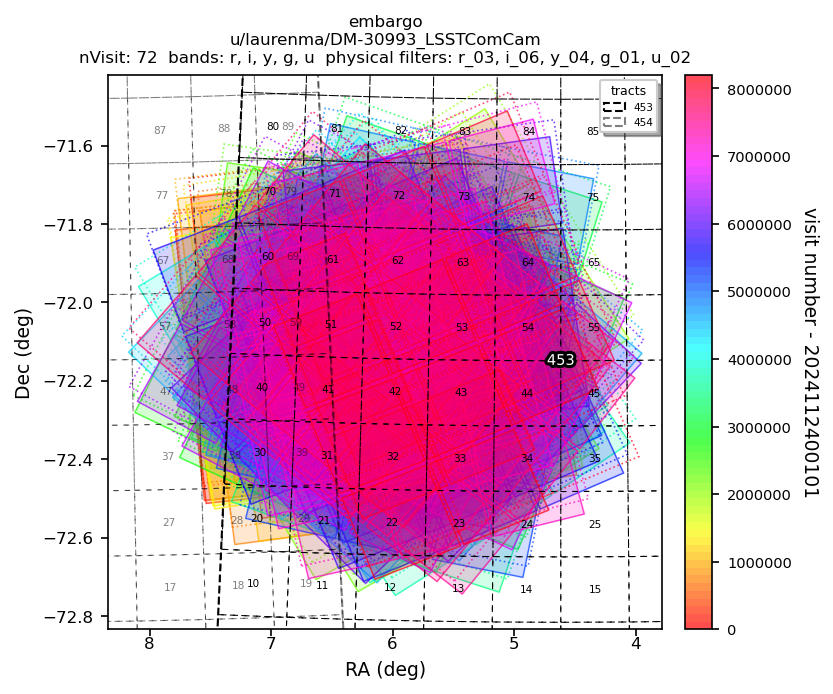
\includegraphics[width=0.3\textwidth]{observations_figures/showVisit_DM-30993_LSSTComCam_453.png}
        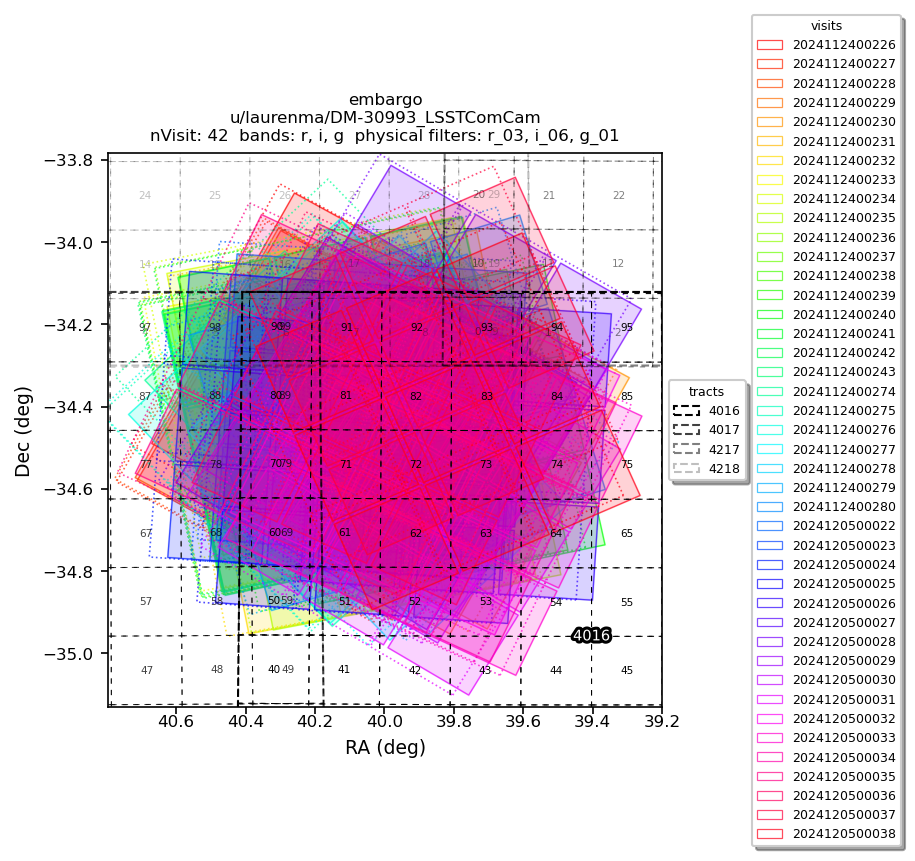
\includegraphics[width=0.3\textwidth]{observations_figures/showVisit_DM-30993_LSSTComCam_4016.png}
        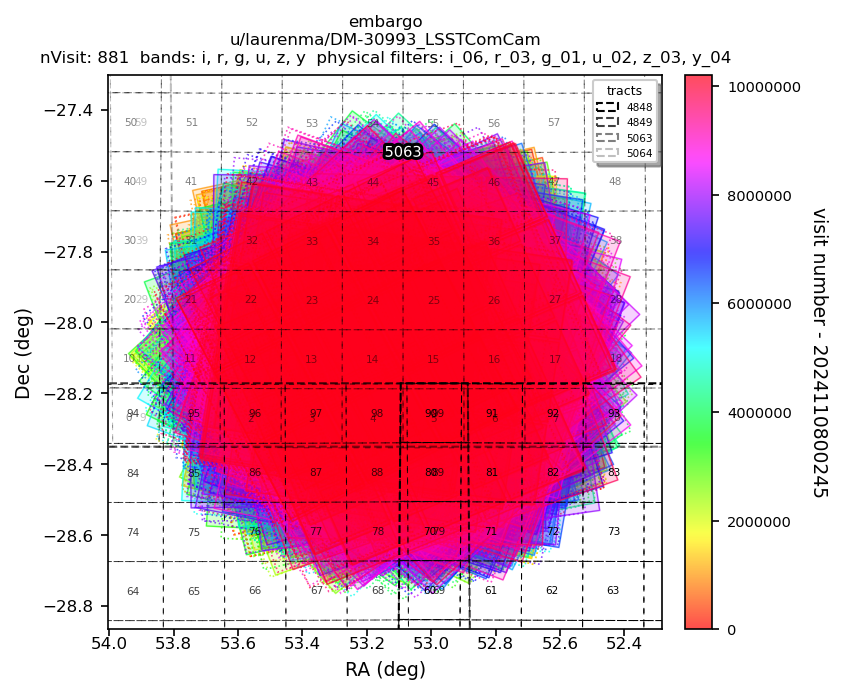
\includegraphics[width=0.3\textwidth]{observations_figures/showVisit_DM-30993_LSSTComCam_5063.png}
        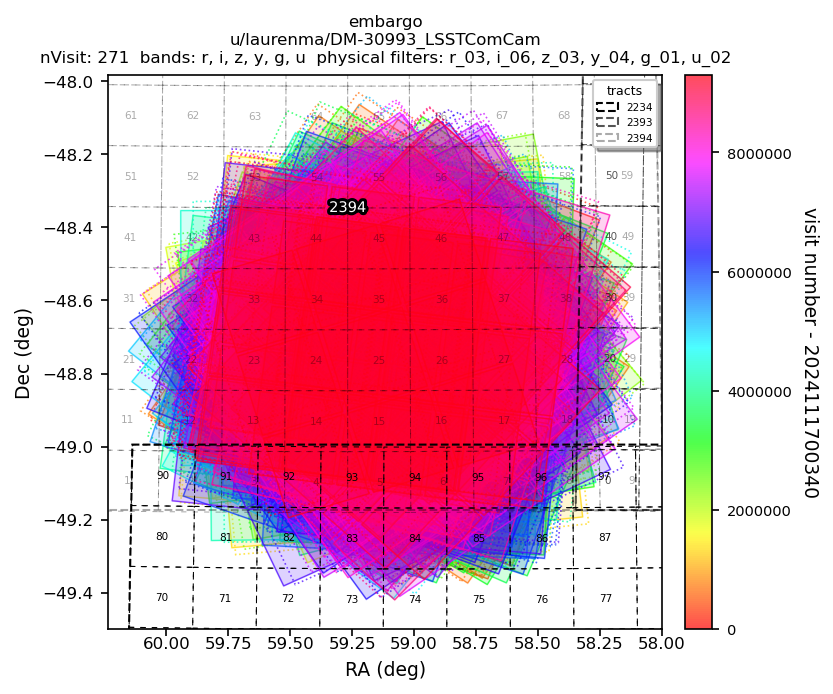
\includegraphics[width=0.3\textwidth]{observations_figures/showVisit_DM-30993_LSSTComCam_2394.png}
        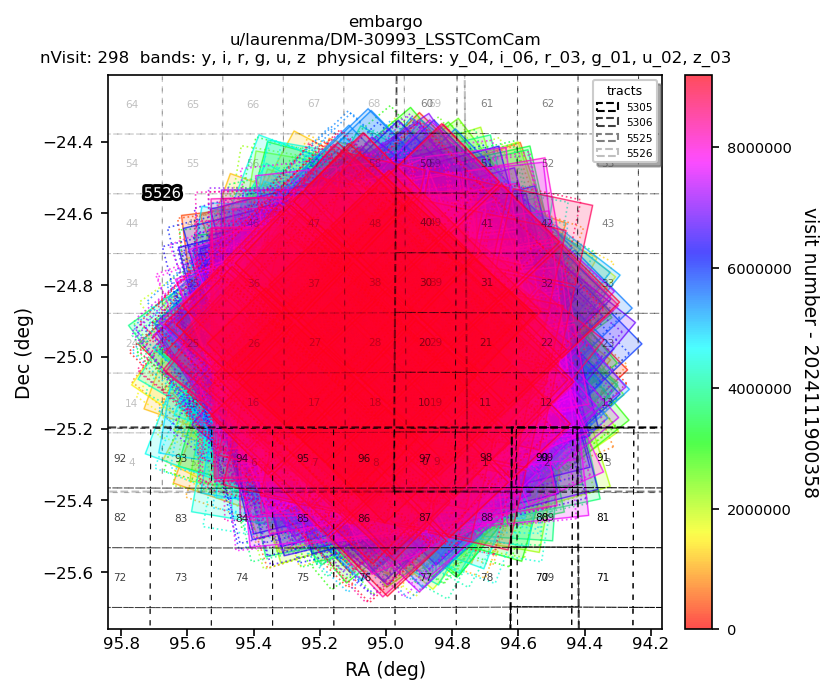
\includegraphics[width=0.3\textwidth]{observations_figures/showVisit_DM-30993_LSSTComCam_5526.png}
        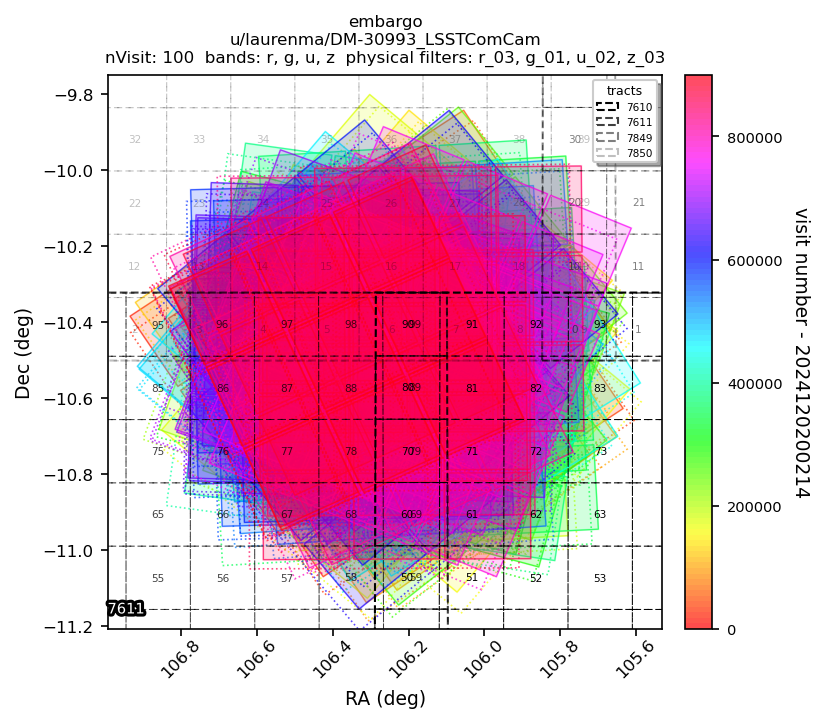
\includegraphics[width=0.3\textwidth]{observations_figures/showVisit_DM-30993_LSSTComCam_7611.png}
    \end{center}
    \caption{Sky coverage for six ComCam Deep Drilling Fields.
    First Row (left to right): 47 Tuc, Fornax dSph, ECDFS.
    Second Row (left to right): EDFS, RubinSV 95 -25, Seagull.}
    \label{fig:comcam_ddf_coverage}
\end{figure}

\begin{figure}
    \begin{center}
      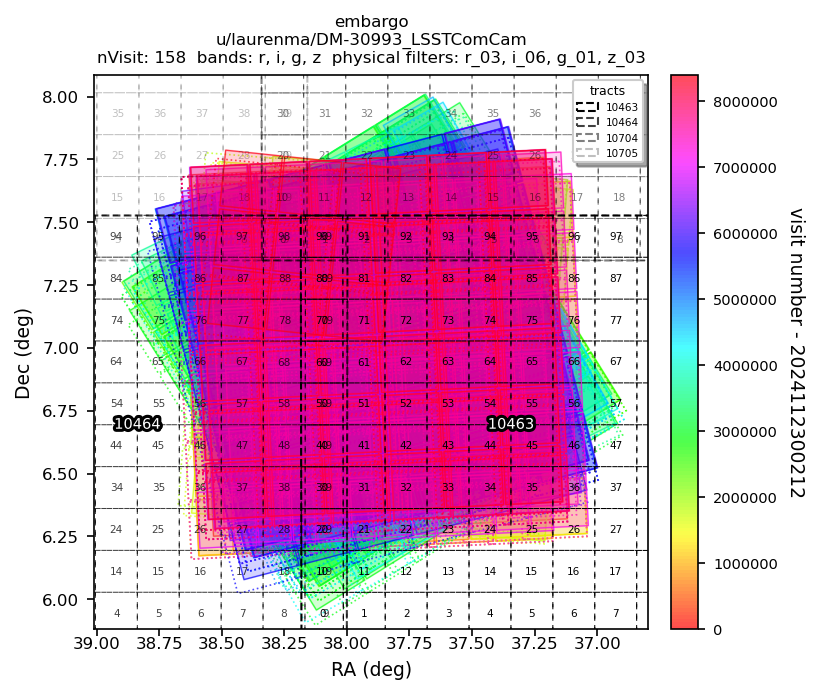
\includegraphics[width=0.3\textwidth]{observations_figures/showVisit_DM-30993_LSSTComCam_10463.png}
    \end{center}
    \caption{Sky coverage for Low Ecliptic Latitude Field (Rubin SV 38 7) during the ComCam on-sky campaign.}
    \label{fig:comcam_ecliptic_coverage}
\end{figure}

\begin{figure}
    \begin{center}
        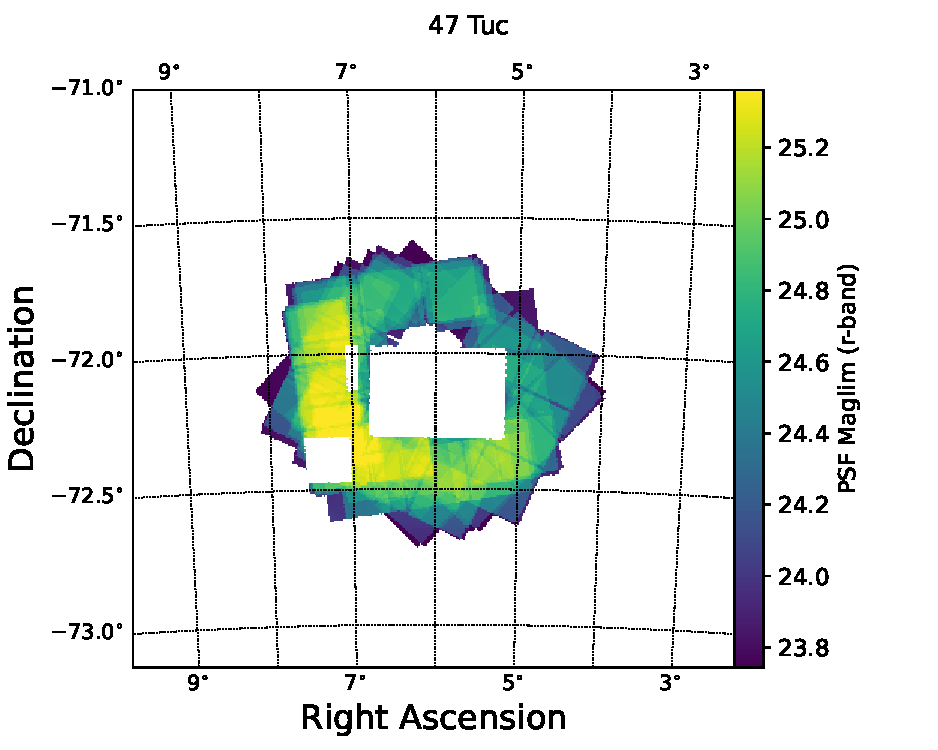
\includegraphics[width=0.32\textwidth]{observations_figures/comcam_psf_maglim_47_tuc_r.pdf}
        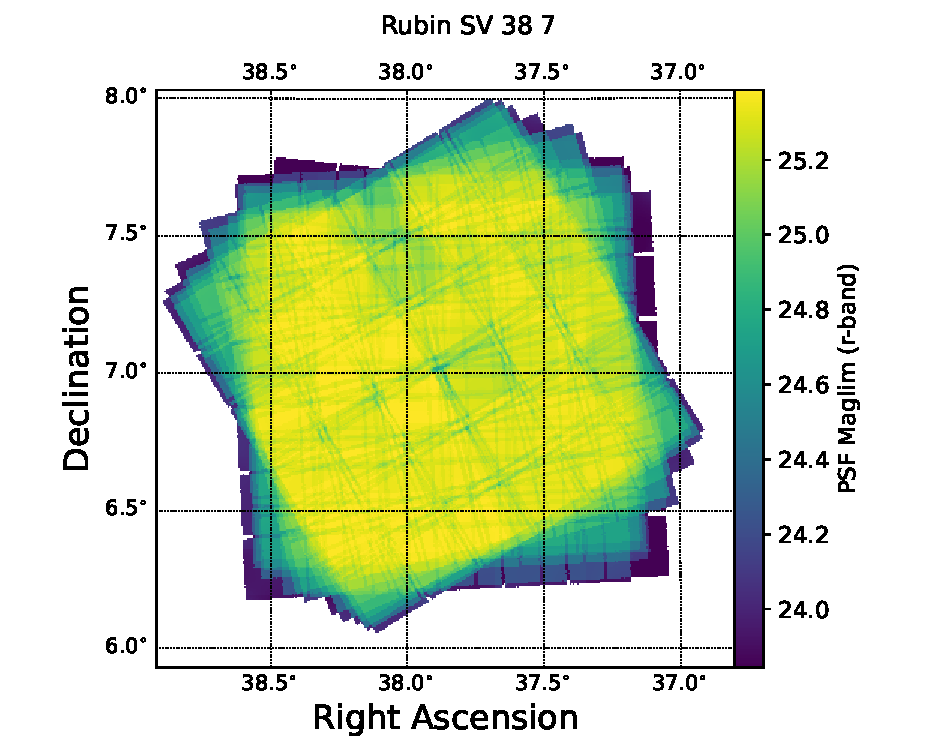
\includegraphics[width=0.32\textwidth]{observations_figures/comcam_psf_maglim_rubin_sv_38_7_r.pdf}
        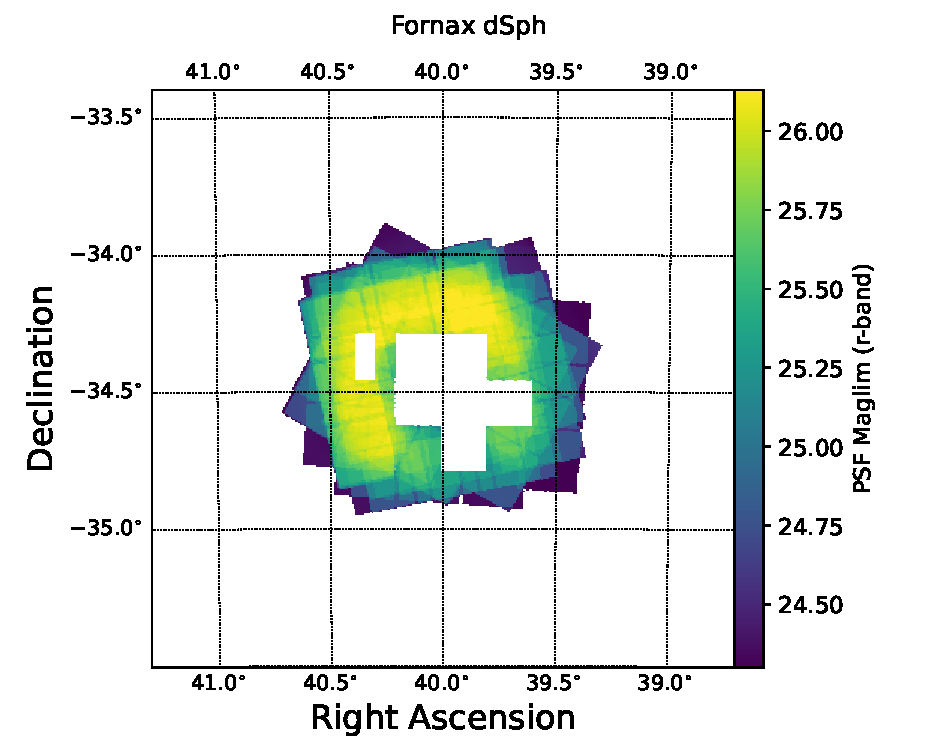
\includegraphics[width=0.32\textwidth]{observations_figures/comcam_psf_maglim_fornax_dsph_r.pdf}
        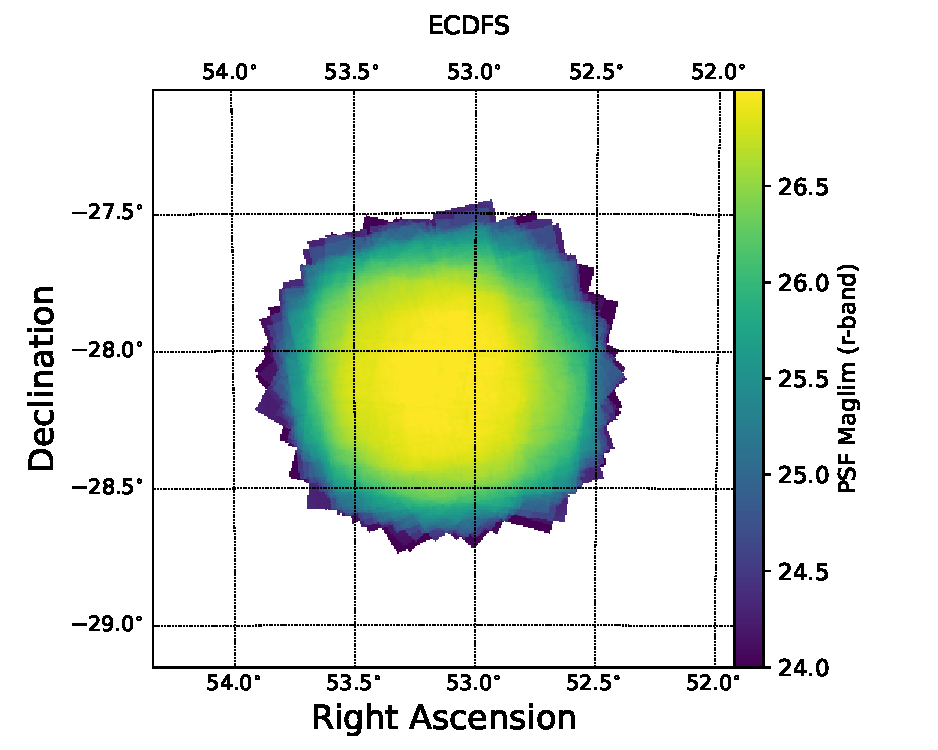
\includegraphics[width=0.32\textwidth]{observations_figures/comcam_psf_maglim_ecdfs_r.pdf}
        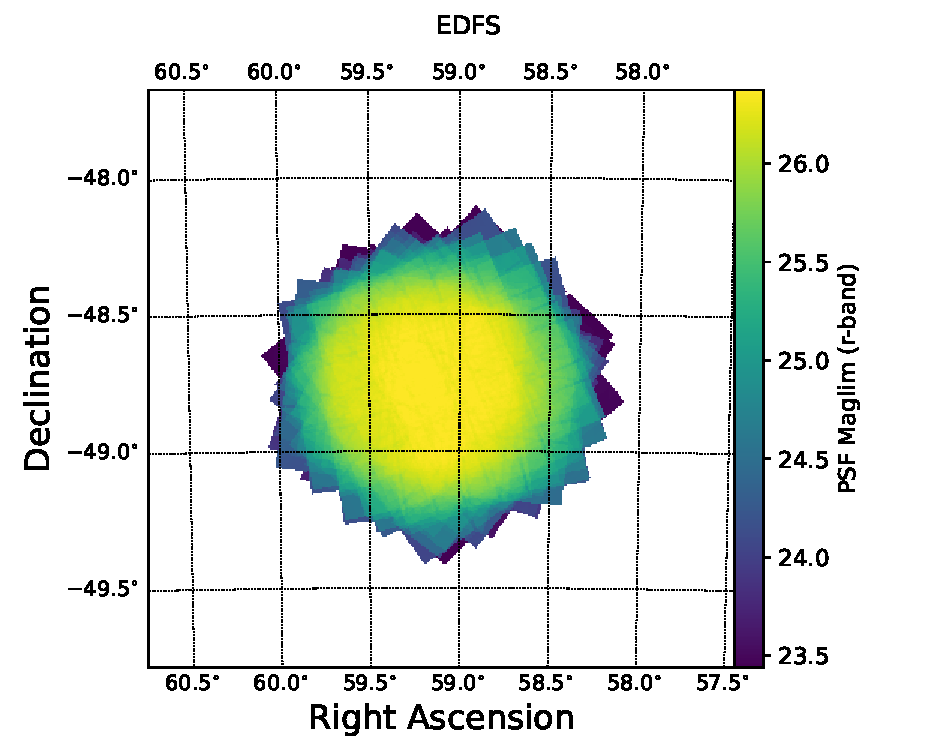
\includegraphics[width=0.32\textwidth]{observations_figures/comcam_psf_maglim_edfs_r.pdf}
        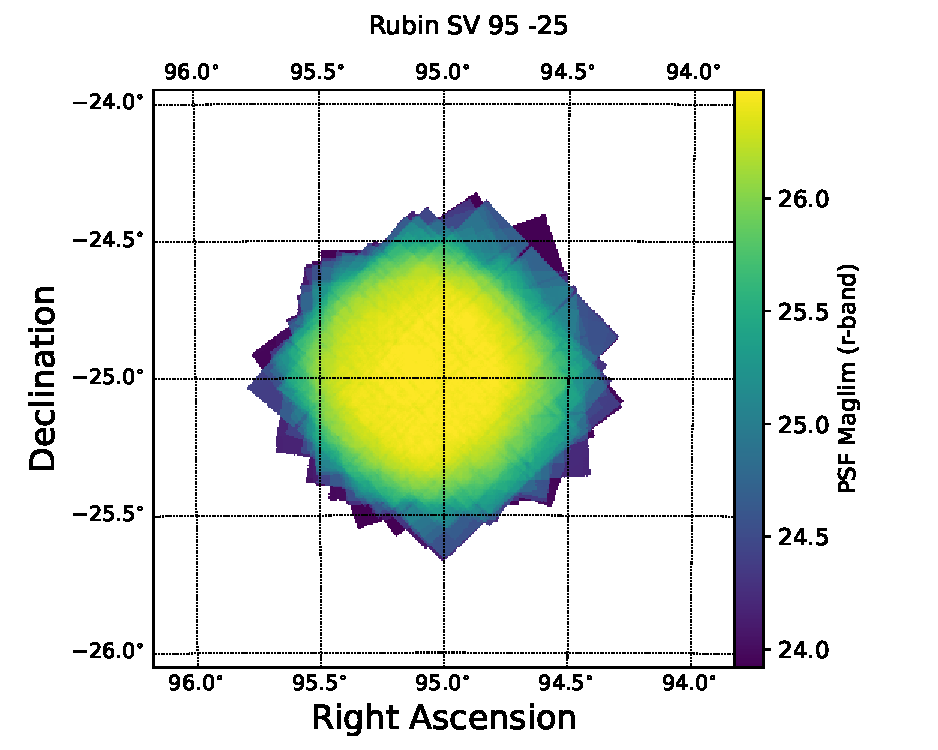
\includegraphics[width=0.32\textwidth]{observations_figures/comcam_psf_maglim_rubin_sv_95_-25_r.pdf}
        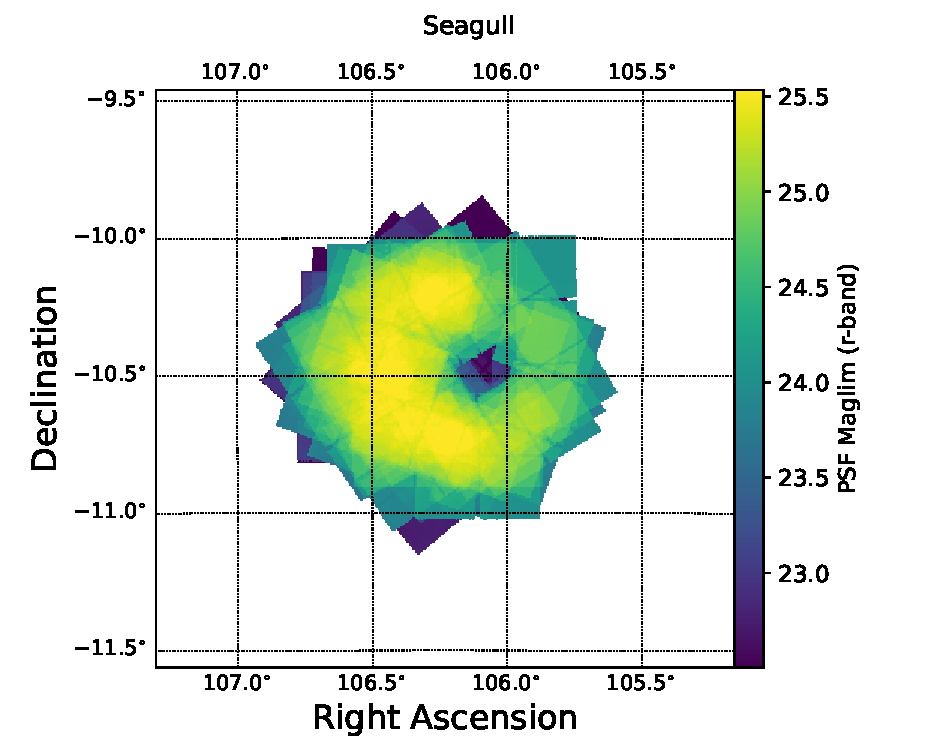
\includegraphics[width=0.32\textwidth]{observations_figures/comcam_psf_maglim_seagull_r.pdf}
    \end{center}
    \caption{Cumulative imaging depth expressed in terms of the $S/N=5$ limiting magnitude for unresolved sources for seven ComCam Deep Drilling Fields.
    First Row (left to right): 47 Tuc, Rubin SV 38 7, Fornax dSph.
    Second Row (left to right): ECDFS, EDFS, RubinSV 95 -25.
    Third Row: Seagull.}
    \label{fig:comcam_ddf_psf_maglim}
\end{figure}



\begin{table*}
    \centering
    \begin{tabular}{@{}lcccccc@{}}
    \textbf{Target} & \textbf{u} & \textbf{g} & \textbf{r} & \textbf{i} & \textbf{z} & \textbf{y} \\
    47 Tuc          &	     6 & 	10 &	33 &	19 &	 0 &     5 \\
    Rubin SV 38 7 	&       0 &    44 & 	55 &	57 &    27 &     0 \\
    Fornax dSph 	&       0 &	 5 &	26 &	13 &	 0 &	 0 \\
    ECDFS 	        &      53 &   230 &   257 &   177 &   177 &	30 \\
    EDFS ComCam 	&      20 &	61 & 	90 &	42 &	42 &	20 \\
    Rubin SV 95 -25 & 	    33 &	86 &	97 &	29 &	60 &	11 \\
    Seagull 	    &      10 &	37 &   	49 &	3  & 	13 & 	 0 \\
    \end{tabular}
    \caption{Band coverage for seven target fields observed for Science Pipelines commissioning during the ComCam on-sky campaign.}
    \label{tab:target_fields_band_coverage}
\end{table*}

\begin{figure}
    \begin{center}
        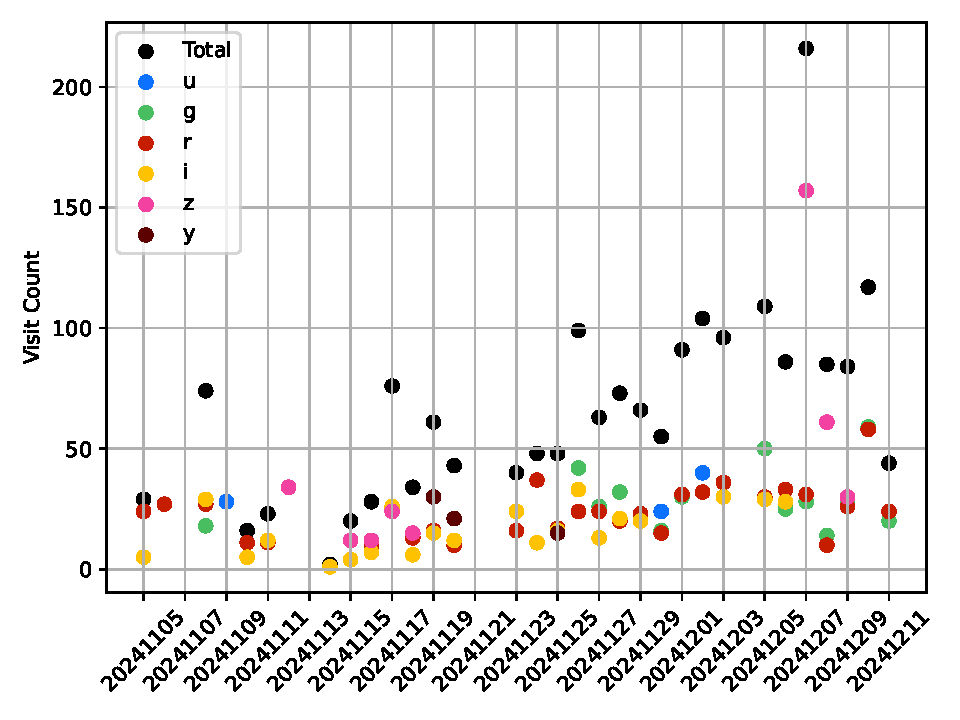
\includegraphics[width=0.7\textwidth]{observations_figures/comcam_science_visit_count_day_obs.pdf}
    \end{center}
    \caption{Distribution of Science Pipelines commissioning observations by \texttt{day\_obs} during the ComCam on-sky campaign.}
    \label{fig:comcam_science_day_obs}
\end{figure}

\begin{figure}
    \begin{center}
        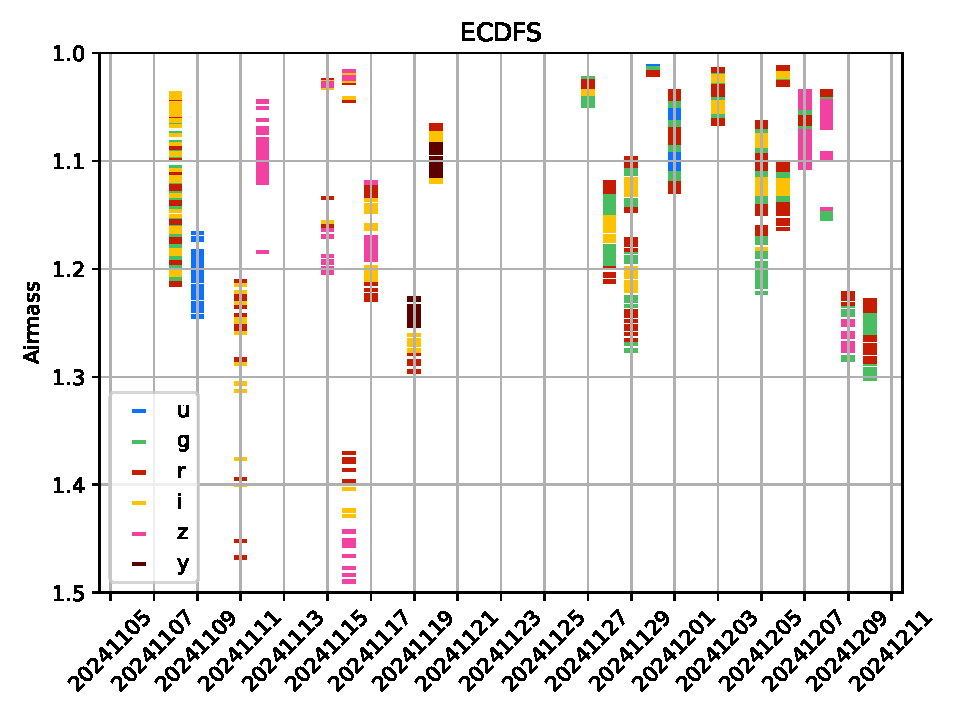
\includegraphics[width=0.7\textwidth]{observations_figures/comcam_science_airmass_day_obs_ecdfs.pdf}
    \end{center}
    \caption{Distribution of Science Pipelines commissioning observations for the ECDFS field during the ComCam on-sky campaign.}
    \label{fig:comcam_science_day_obs_ecdfs}
\end{figure}